\subsection{Subpaso 1-A: Iniciar estadísticas por años}
	En la configuración de las estadísticas se tiene que seleccionar el 
	inciso \textbf{Años} y el año o años(puede seleccionar uno o mas) que desea 
	consultar.
		
	\begin{figure}[hbtp]

	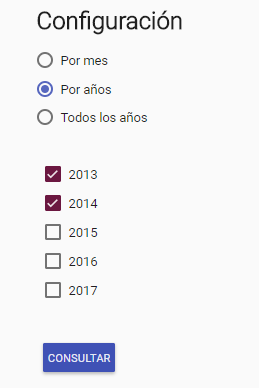
\includegraphics[scale=0.5]{images/Interfaz/IUGS15_configuracioAnos.PNG}
	\caption{Configuración por Años }
	\end{figure}
	A continuación se aprieta el botón \textbf{Consultar}
	
\subsection{Subpaso 1-B: Muestra de Estadísticas}
	Se mostrará la siguiente interfaz con las siguientes estadísticas:
	\begin{figure}[hbtp]
		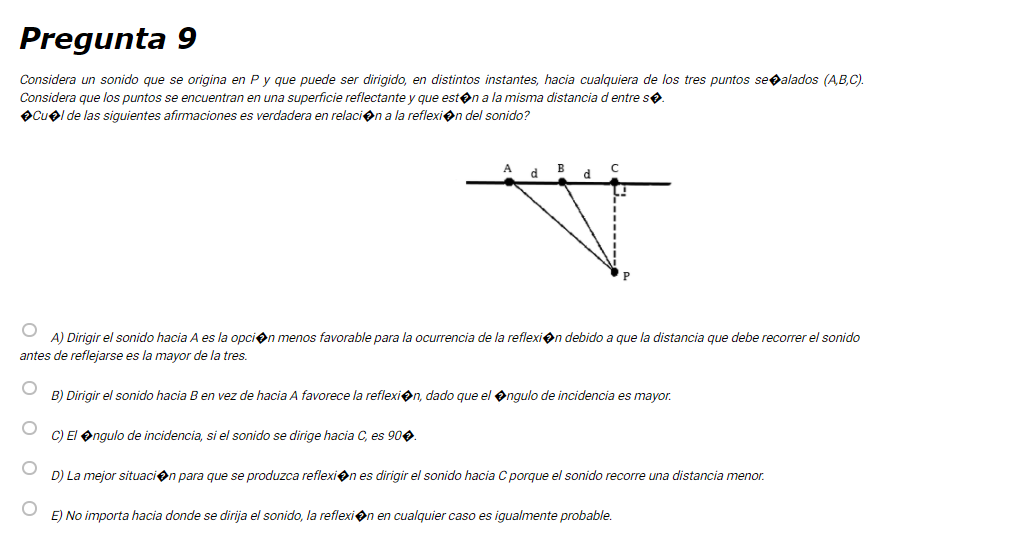
\includegraphics[scale=0.3]{images/Interfaz/IUGS15_estadisticasAnos.PNG}
		\caption{Pagina general de Estadísticas por Años}
	\end{figure}	
	
\begin{itemize}
	\item  Las estadísticas que se mostraran son las siguientes:
	\begin{enumerate}
		
		\item Número de préstamos de recursos
		\begin{figure}[hbtp]
	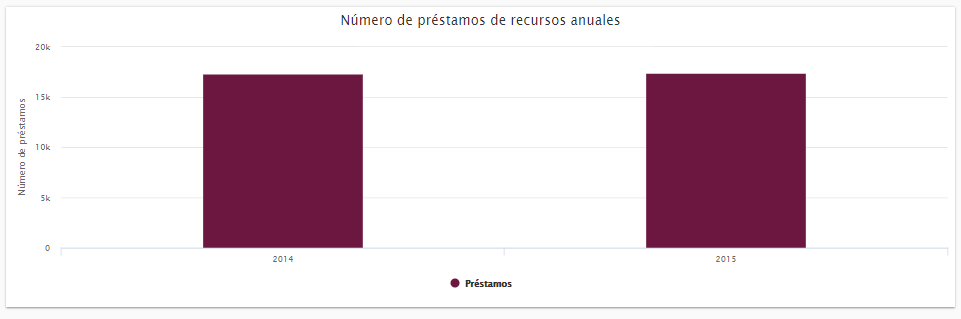
\includegraphics[scale=0.7]{images/Interfaz/IUGS15_recursosAnos.PNG}
	\caption{Número de préstamos de recursos}
	\end{figure}
	
	\item Número de préstamos de salas
	\begin{figure}[hbtp]
	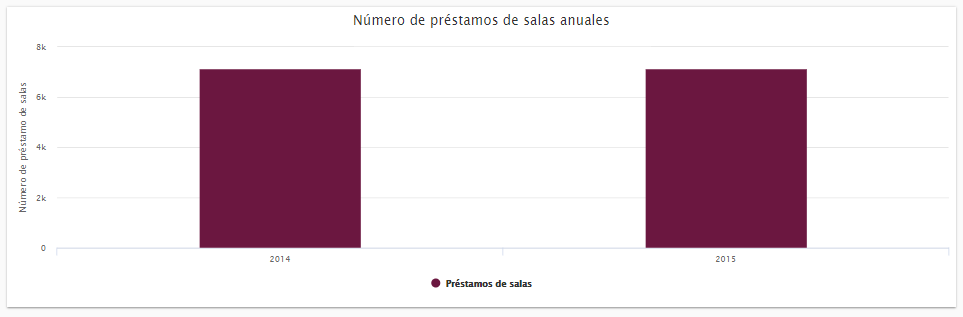
\includegraphics[scale=0.7]{images/Interfaz/IUGS15_salasAnos.PNG}
	\caption{Número de préstamos de salas}
	\end{figure}
	
	\item Número de préstamos de salas
	\begin{figure}[hbtp]
	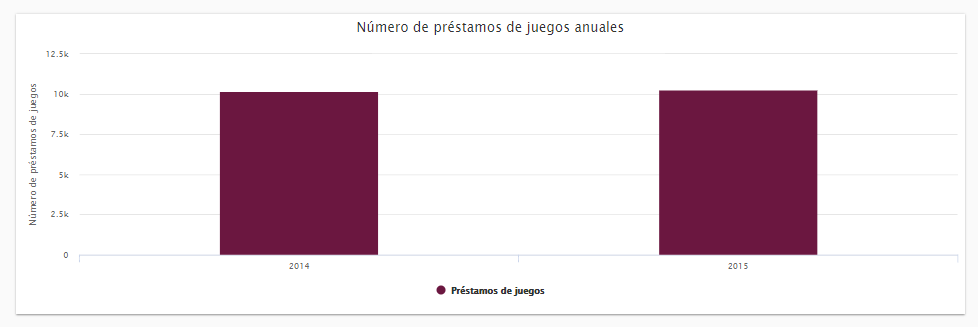
\includegraphics[scale=0.7]{images/Interfaz/IUGS15_juegosAnos.PNG}
	\caption{Número de préstamos de juegos}
	\end{figure}
	
	\item Encuesta de calidad: promedio
	\begin{figure}[hbtp]
	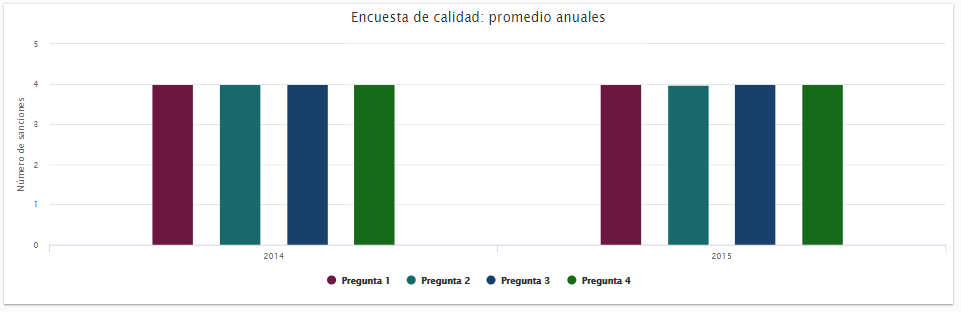
\includegraphics[scale=0.7]{images/Interfaz/IUGS15_encuestaCalidadAnos.PNG}
	\caption{Encuesta de calidad: promedio}
	\end{figure}
	
	\item Número de sanciones 
	\begin{figure}[hbtp]
	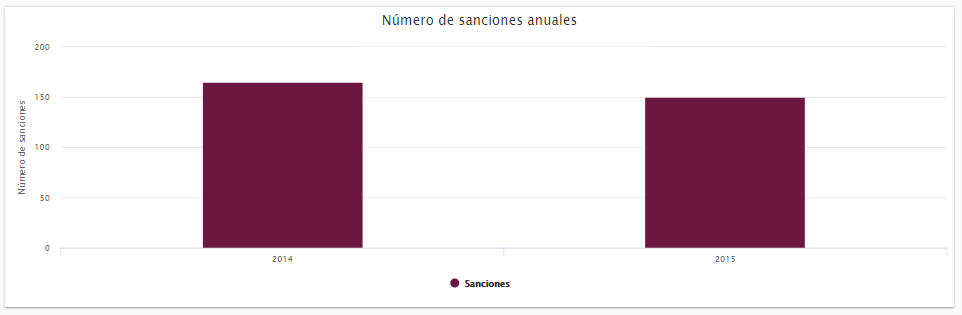
\includegraphics[scale=0.7]{images/Interfaz/IUGS15_sancionesAnos.PNG}
	\caption{Número de sanciones}
	\end{figure}
	
	\end{enumerate}
	
\end{itemize}